\documentclass[14pt]{extarticle}
\usepackage[a4paper, left=2cm, right=2cm, top=1.5cm, bottom=2cm]{geometry}
\usepackage[utf8]{inputenc}
\usepackage[T2A]{fontenc}
\usepackage[russian]{babel}
\usepackage{indentfirst}
\usepackage{enumitem}
\usepackage{amsmath,amsfonts,amssymb}
\usepackage{icomma}
\usepackage{graphicx}
\usepackage{framed}
\usepackage{caption}
\usepackage{float}
\usepackage{titletoc}
\usepackage{hyperref}
\usepackage{paratype}
\renewcommand{\rmdefault}{PTSans-TLF}


\begin{document}
	
	\thispagestyle{empty}
	
	\begin{center}
		
		\textbf{Санкт-Петербургский политехнический университет}\\
		\vspace{2cm}
		
		Направление подготовки \\
		\large <<01.03.02 Прикладная математика и информатика>>\\
		
		\vspace{7cm}
		
		Отчет по лабораторной работе №6:\\
		\vspace{0.2cm}
		\textbf{\LARGE Решение задачи Коши для ОДУ 1 порядка методами Адамса}
		
		\vspace{6cm}
		
		\begin{flushleft}
			Выполнил студент гр. 5030102/40003 \hfill Т.Р. Абдуллин\\
			Преподаватель: \hfill К.Н. Козлов\\
		\end{flushleft}
		
		\vspace{3cm}
		
		Санкт-Петербург\\
		2026
	\end{center}
	
	%-------- the beginning of report --------
	
	\tableofcontents
	%-------- the first point --------
	\newpage
	\section{\Large \underline{Формулировка задачи и ее формализация}}
	\subsection{Формулировка задачи}
	
	Требуется численно решить задачу Коши для обыкновенного
	дифференциального уравнения первого порядка на отрезке
	$\left[\frac{\pi}{2}, 2\pi\right]$
	методом Эйлера с пересчётом (методом трапеций).
	
	Исследуемое уравнение имеет вид:
	
	\[
	y = x(y' - x\cos x)
	\]
	
	Начальное условие:
	
	\[
	y\left(\frac{\pi}{2}\right)=\frac{\pi}{2}
	\]
	
	Точное решение задачи:
	
	\[
	y(x)=x\sin x
	\]
	
	Требуется:
	
	\begin{itemize}
		\item реализовать метод Эйлера с пересчётом;
		\item организовать итерационный процесс пересчёта
		до достижения заданной точности;
		\item исследовать точность численного метода;
		\item построить графики численного и точного решений;
		\item исследовать зависимость фактической погрешности
		от заданной точности.
	\end{itemize}
	
	\subsection{Формализация задачи}
	
	Преобразуем исходное уравнение к стандартной форме задачи Коши.
	
	Исходное уравнение:
	
	\[
	y = x(y' - x\cos x)
	\]
	
	Разделим на $x$:
	
	\[
	\frac{y}{x}=y'-x\cos x
	\]
	
	Выразим производную:
	
	\[
	y'=\frac{y}{x}+x\cos x
	\]
	
	Тогда задача Коши принимает вид:
	
	\[
	\begin{cases}
		y' = f(x,y), \\
		y(x_0)=y_0,
	\end{cases}
	\]
	
	где
	
	\[
	f(x,y)=\frac{y}{x}+x\cos x
	\]
	
	начальные данные:
	
	\[
	x_0=\frac{\pi}{2},
	\qquad
	y_0=\frac{\pi}{2}
	\]
	
	точное решение:
	
	\[
	y(x)=x\sin x
	\]
	
	Рассматриваемый отрезок:
	
	\[
	x\in\left[\frac{\pi}{2},2\pi\right]
	\]
	
	%-------- the second point --------
	
	\newpage
	\section{\Large \underline{Алгоритм метода}}
	
	\subsection{Псевдокод метода}
	
	Метод Эйлера с пересчётом относится к неявным
	одношаговым методам.
	
	Предиктор вычисляется явным методом,
	после чего выполняется итерационный пересчёт.
	
	Формулы метода:
	
	\[
	y_{n+1}^{(0)}
	=
	y_n+h f(x_n,y_n)
	\]
	
	\[
	y_{n+1}^{(k+1)}
	=
	y_n
	+
	\frac{h}{2}
	\left[
	f(x_n,y_n)
	+
	f(x_{n+1},y_{n+1}^{(k)})
	\right]
	\]
	
	Критерий остановки итераций:
	
	\[
	\left|
	y_{n+1}^{(k+1)}
	-
	y_{n+1}^{(k)}
	\right|
	<
	\varepsilon
	\]
	
	Псевдокод алгоритма:
	
	\begin{enumerate}
		\item Задать:
		\[
		a,\ b,\ h,\ \varepsilon,\ y_0
		\]
		
		\item Положить:
		\[
		x_0=a
		\]
		
		\item Пока:
		\[
		x_n<b
		\]
		
		выполнять:
		
		\begin{enumerate}
			\item Вычислить предиктор:
			
			\[
			y_{n+1}^{(0)}
			\]
			
			\item Выполнить итерационный пересчёт:
			
			\[
			y_{n+1}^{(k+1)}
			=
			y_n
			+
			\frac{h}{2}
			\left[
			f(x_n,y_n)
			+
			f(x_{n+1},y_{n+1}^{(k)})
			\right]
			\]
			
			\item Проверить условие:
			
			\[
			\left|
			y_{n+1}^{(k+1)}
			-
			y_{n+1}^{(k)}
			\right|
			<
			\varepsilon
			\]
			
			\item Если условие выполнено,
			принять:
			
			\[
			y_{n+1}=y_{n+1}^{(k+1)}
			\]
			
			\item Перейти к следующему шагу.
		\end{enumerate}
	\end{enumerate}
	
	\subsection{Условия применимости метода}
	
	Для применимости метода Эйлера с пересчётом
	необходимо выполнение следующих условий:
	
	\begin{enumerate}
		\item Функция
		\[
		f(x,y)
		\]
		должна быть непрерывна
		в рассматриваемой области.
		
		\item Частная производная
		\[
		\frac{\partial f}{\partial y}
		\]
		должна быть непрерывна.
		
		\item Для сходимости итерационного процесса
		пересчёта необходимо выполнение условия сжатия:
		
		\[
		\left|
		\frac{h}{2}
		\frac{\partial f}{\partial y}
		\right|
		<1
		\]
		
		\item Шаг интегрирования должен быть
		достаточно малым для обеспечения устойчивости
		и сходимости метода.
		
		\item Начальная точка должна принадлежать
		области определения функции.
	\end{enumerate}
	
	%-------- the third point --------
	
	\section{\Large \underline{Проверка условий применимости}}
	
	\begin{figure}[H]
		\centering
		\begin{framed}
			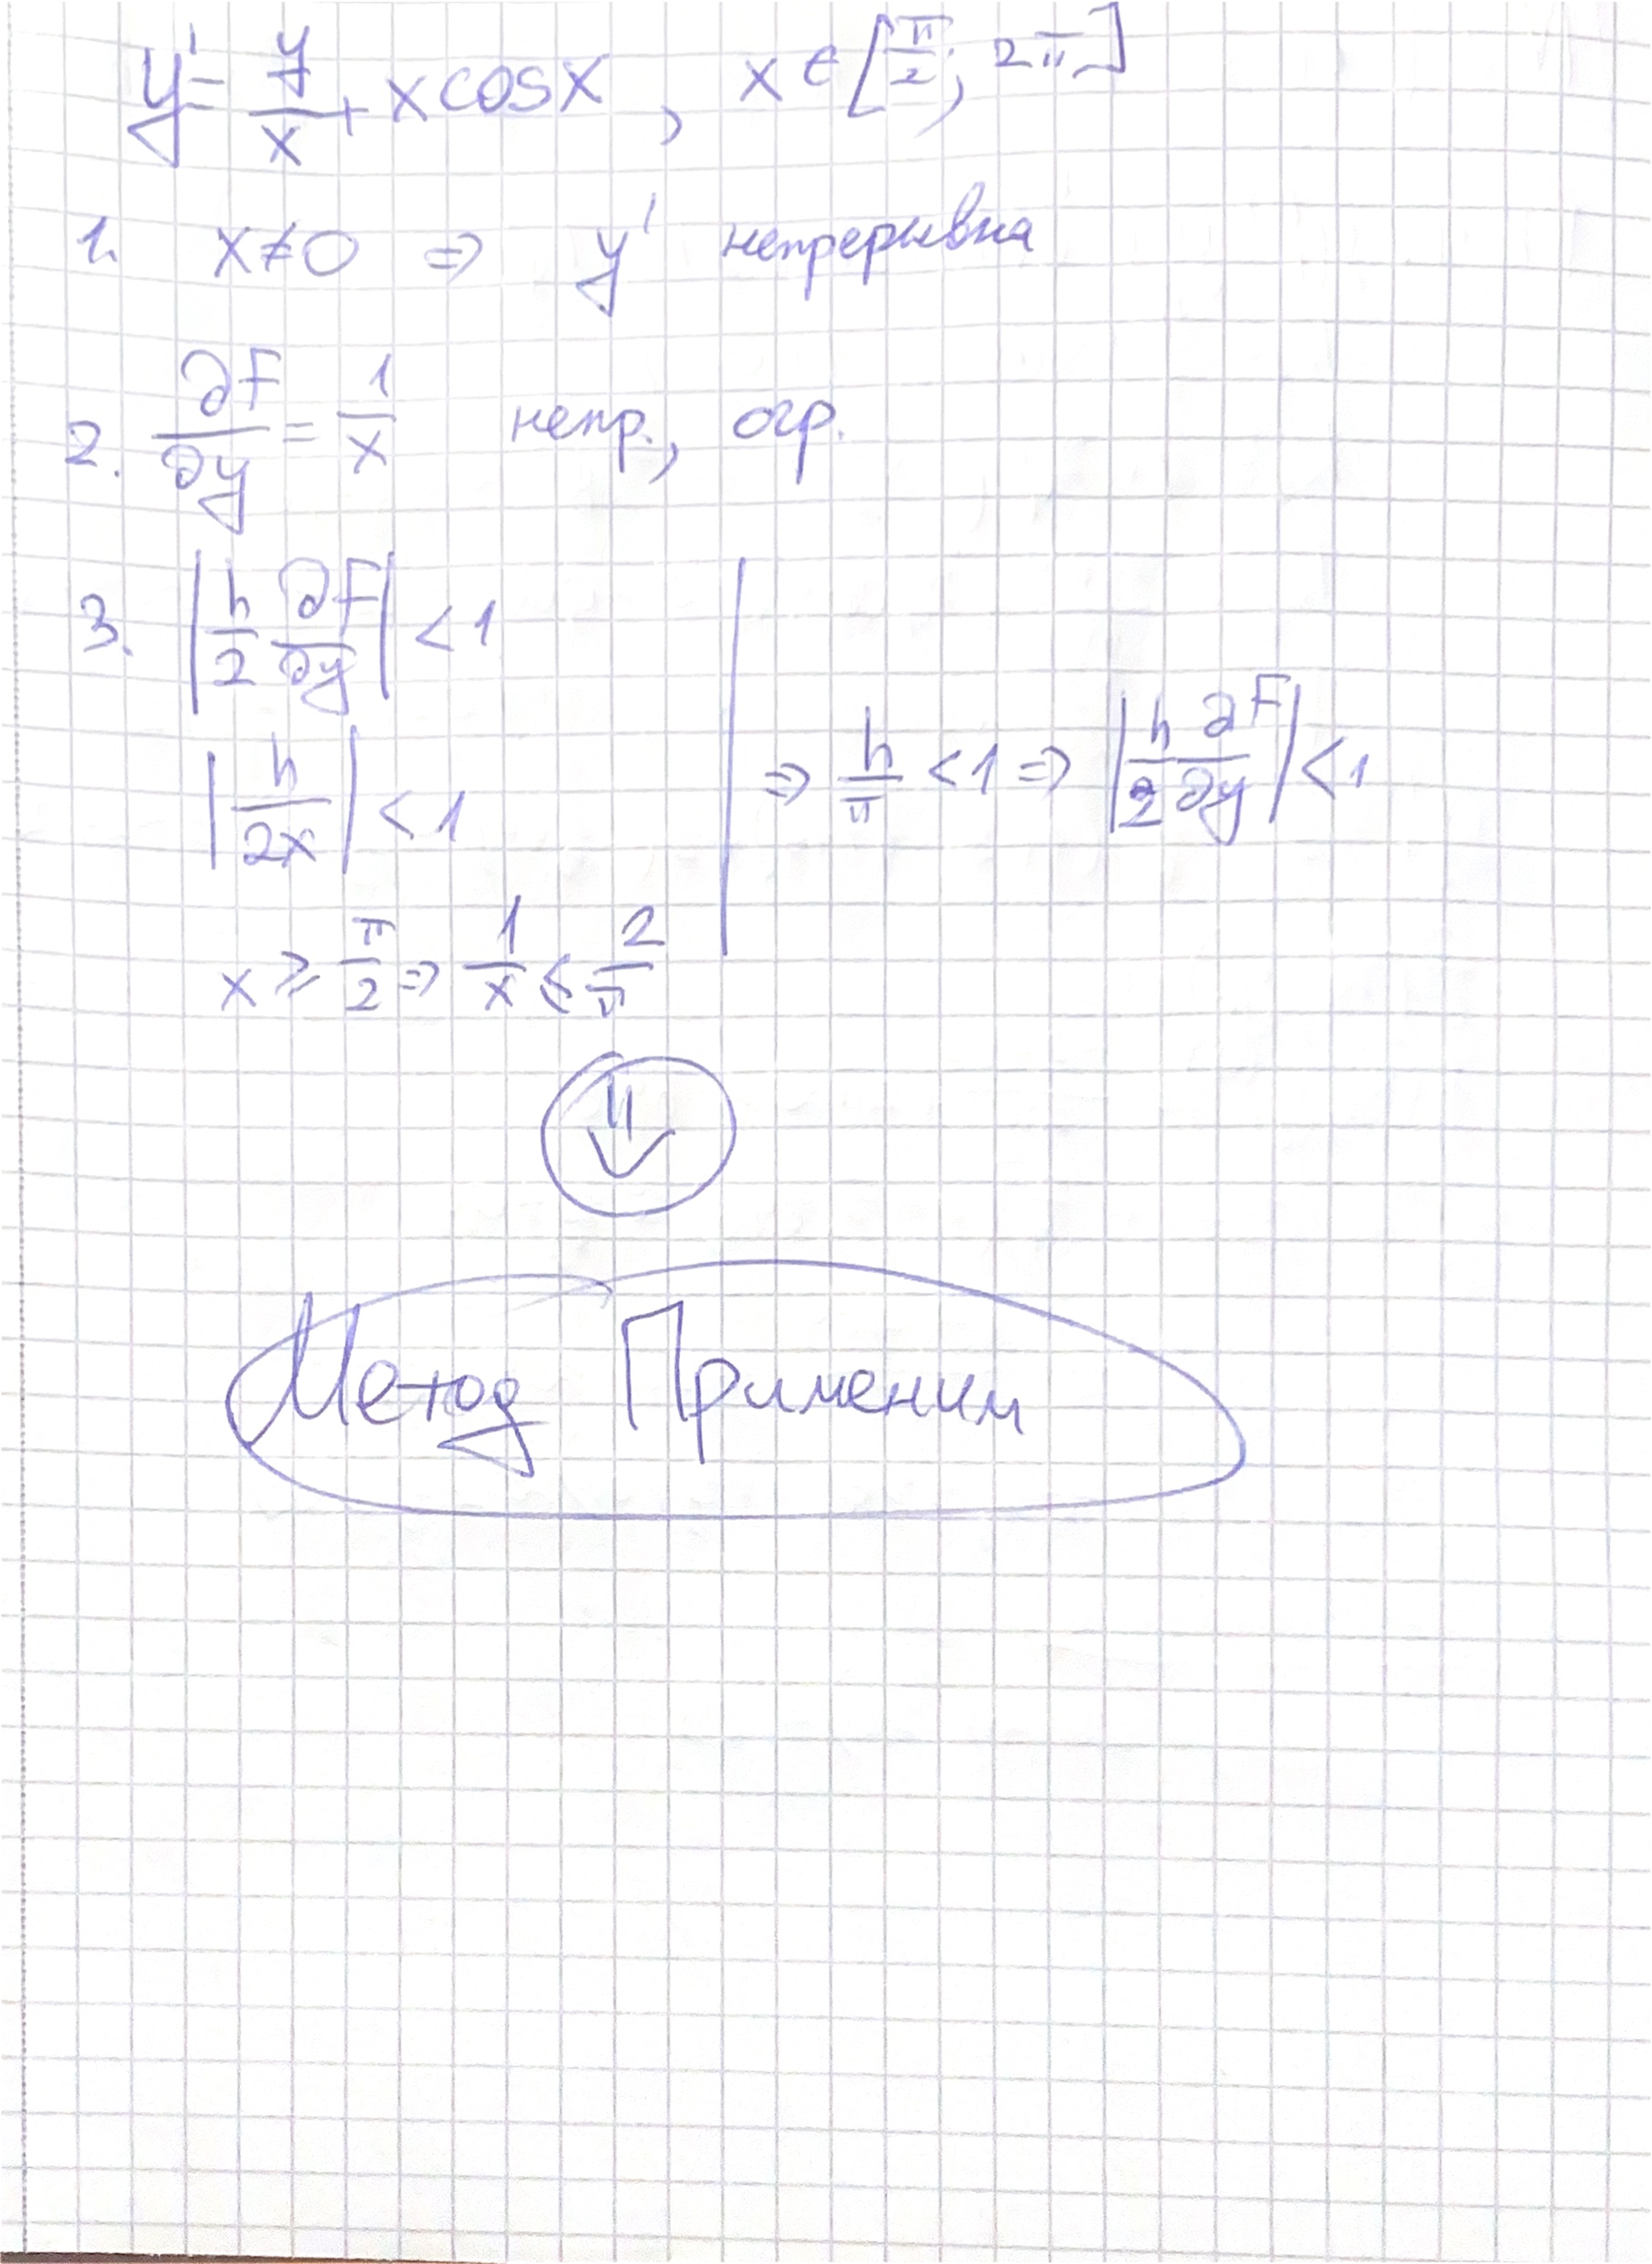
\includegraphics[width=0.9\linewidth]{../data/check.pdf}
			\caption{Проверка условий применимости}
			\label{fig:check}
		\end{framed}
	\end{figure}
	
	
	%-------- the fourth point --------
	
	\newpage
	\section{\Large \underline{Тестовый пример}}
	
	\begin{figure}[H]
		\centering
		\begin{framed}
			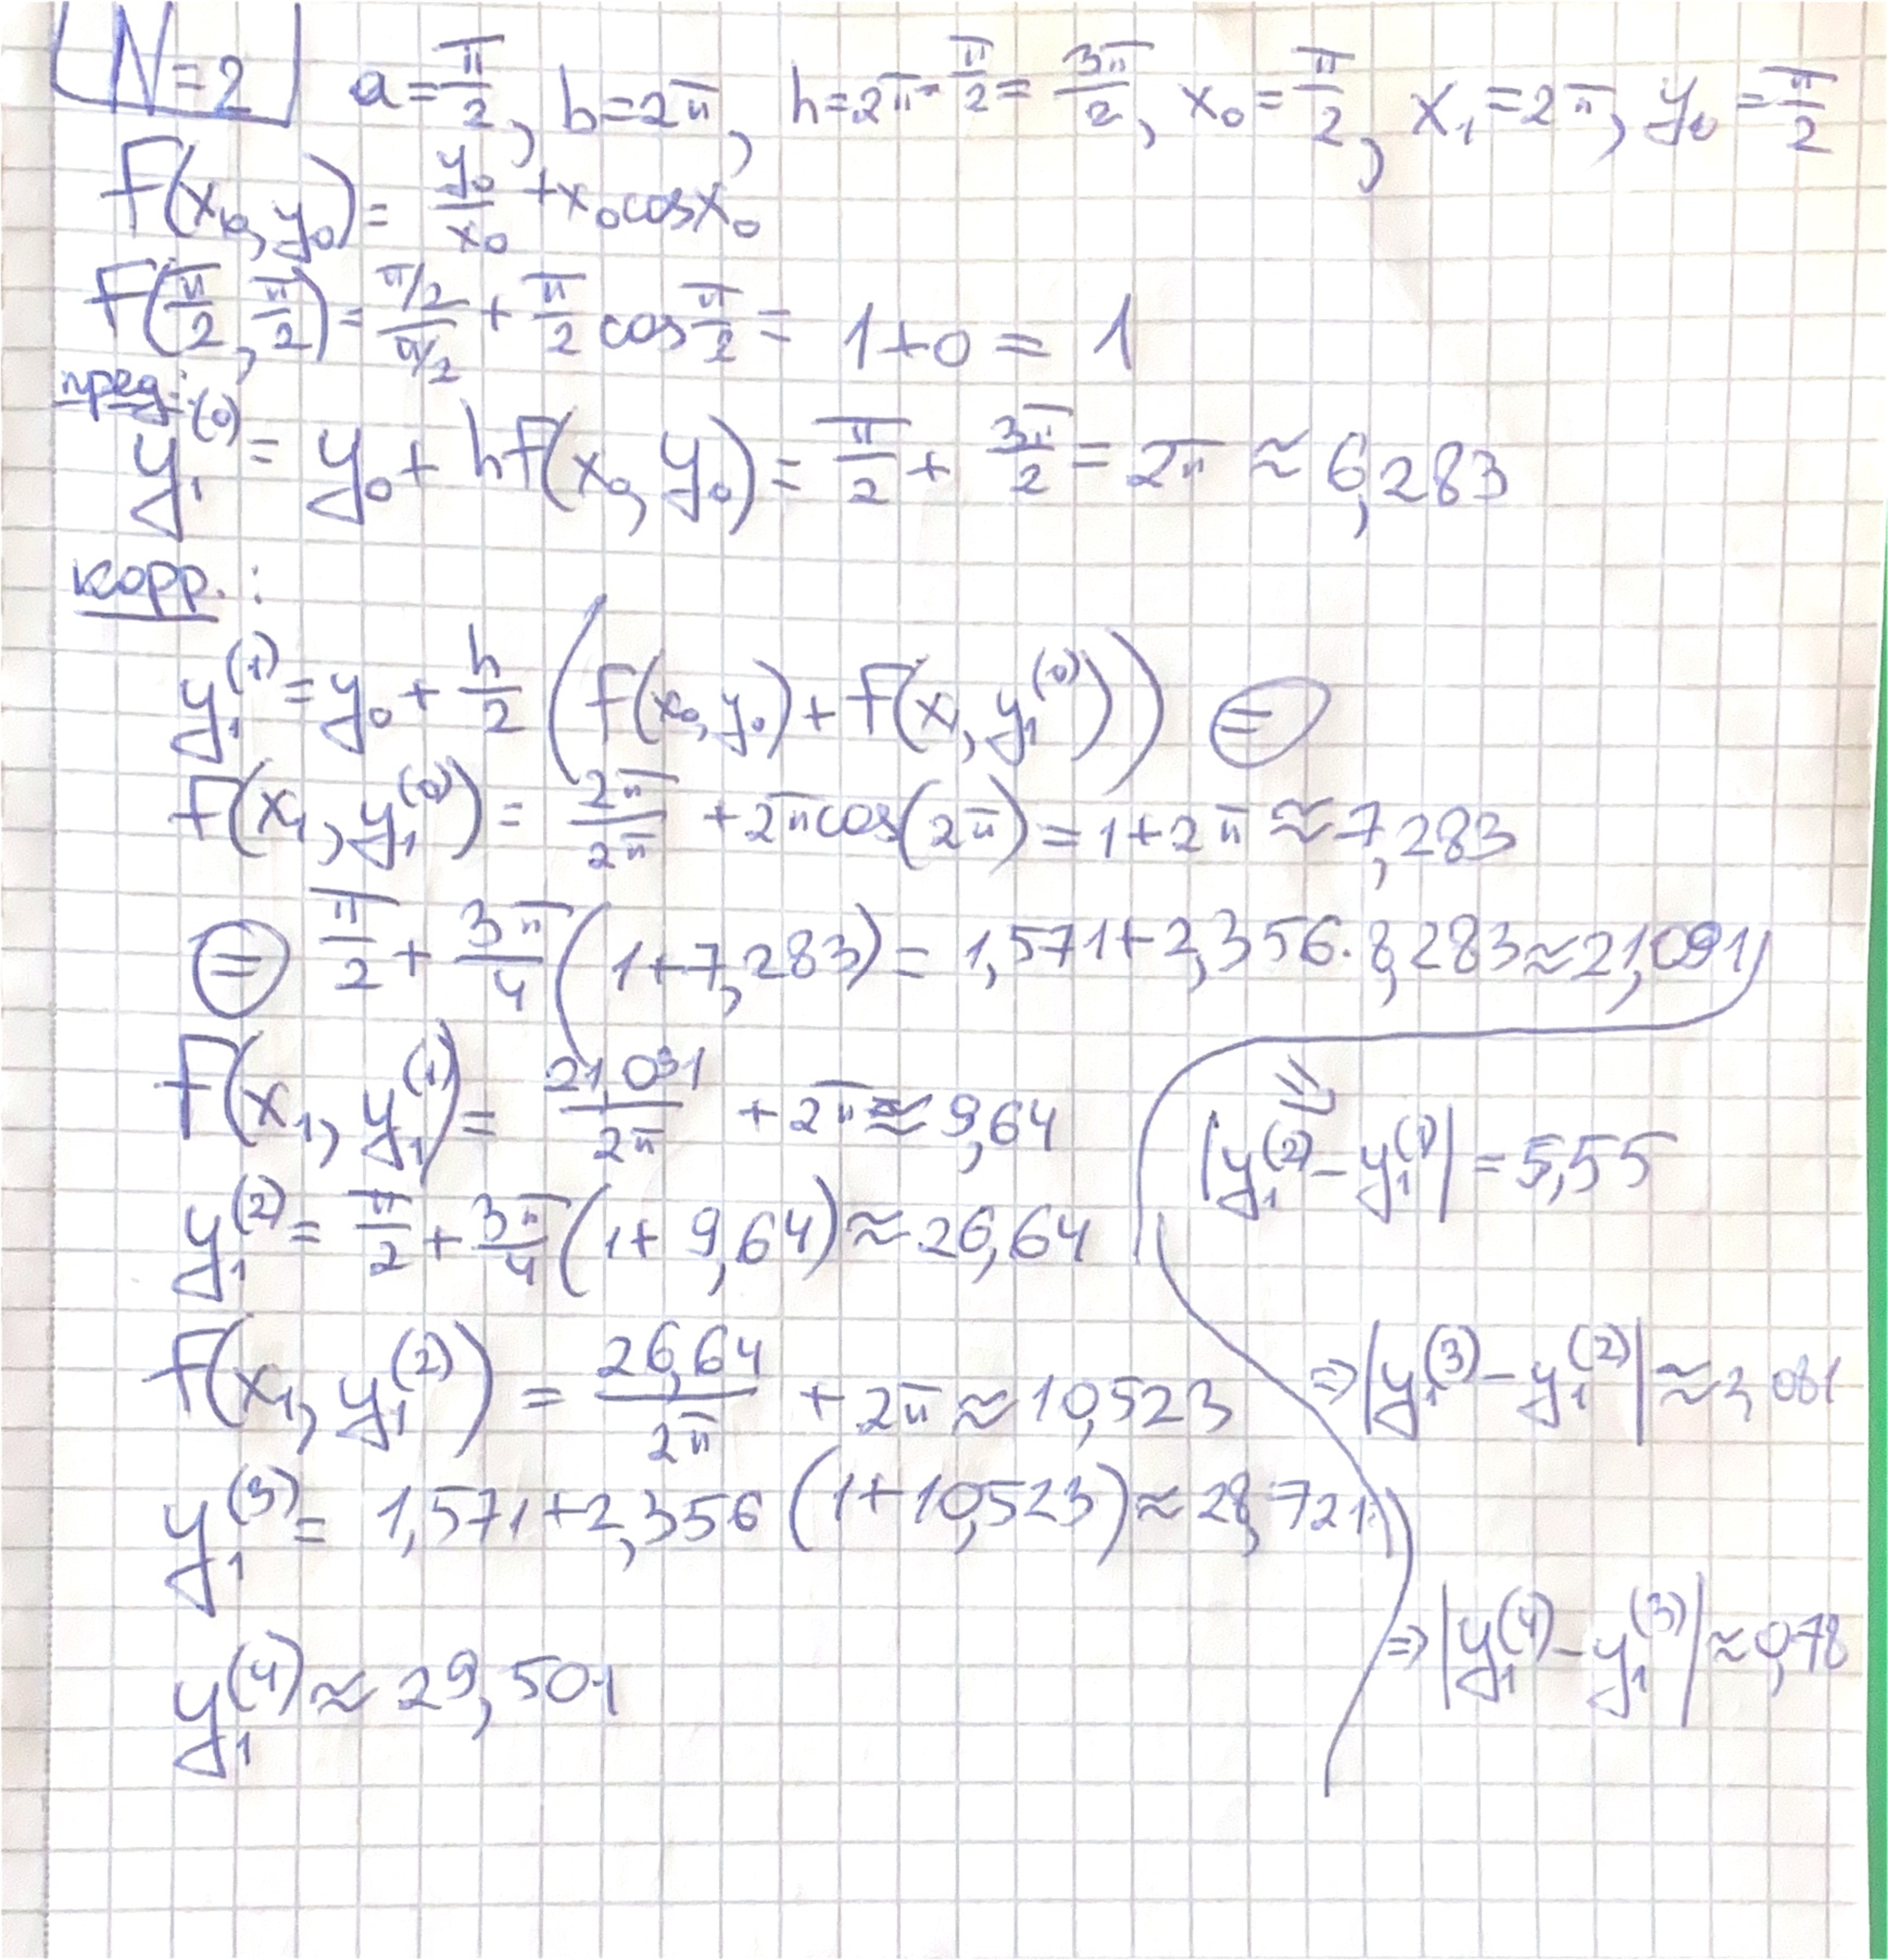
\includegraphics[width=0.9\linewidth]{../data/test_example.pdf}
			\caption{Тестовый пример}
			\label{fig:test}
		\end{framed}
	\end{figure}
	
	Видно, что значение корректора сходится к определенному значению, хоть оно и далеко от точного ($y_{exact} = 0, y \approx 30$) в связи с большим шагом ($N = 2, h = \frac{3\pi}{2}$)
	
	
	
	%-------- the fifth point --------
	
	\newpage
	\section{\Large \underline{Подготовка контрольных тестов}}
	
	Для проверки корректности реализации
	используется задача,
	имеющая известное аналитическое решение.
	
	Исследуемая задача:
	
	\[
	y'=\frac{y}{x}+x\cos x
	\]
	
	Начальное условие:
	
	\[
	y\left(\frac{\pi}{2}\right)=\frac{\pi}{2}
	\]
	
	Точное решение:
	
	\[
	y(x)=x\sin x
	\]
	
	Контроль осуществляется следующим образом:
	
	\begin{enumerate}
		\item Вычисляется численное решение.
		\item В узлах сетки вычисляется точное решение.
		\item Определяется абсолютная погрешность:
		
		\[
		e_i=
		|y_i^{num}-y_i^{exact}|
		\]
		
		\item Определяется максимальная ошибка:
		
		\[
		E=
		\max_i e_i
		\]
	\end{enumerate}
	
	Для исследования метода используются:
	
	\begin{itemize}
		\item различные шаги интегрирования;
		\item различные значения точности
		итерационного пересчёта.
	\end{itemize}
	
	%-------- the sixth point --------
	
	\section{\Large \underline{Модульная структура программы}}
	
	\begin{itemize}
		\item \textbf{function} — вычисление функции $f(x)$
		\begin{itemize}
			\item вход: $x$
			\item выход: $f(x)$
		\end{itemize}
		
		\item \textbf{euler} — метод эйлера
		\begin{itemize}
			\item вход: $a, b, \varepsilon$
			\item выход: вектор точек решения.
		\end{itemize}
	\end{itemize}
	
	%-------- the eighth point --------
	
	\newpage
	\section{\Large \underline{Численный анализ решения задачи}}
	
	\begin{enumerate}[label*=\arabic*), align=left, leftmargin=*, itemindent=1.5em, listparindent=1.5em, parsep=0pt]
		\begin{figure}[H]
			\centering
			\begin{framed}
				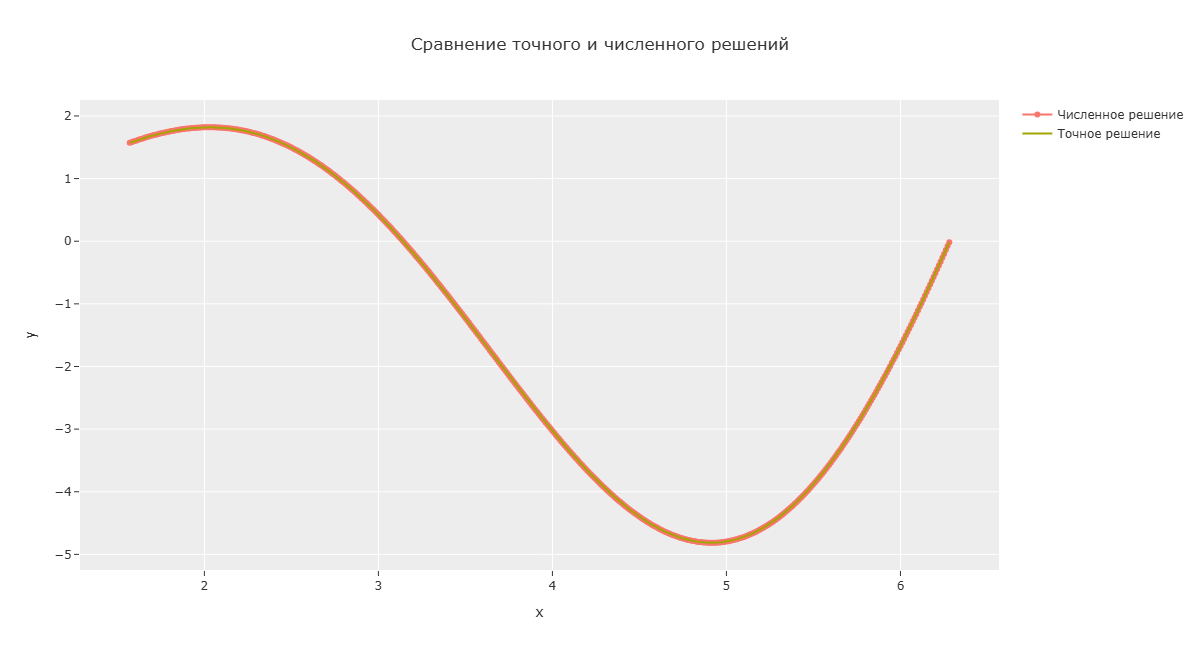
\includegraphics[width=0.9\linewidth]{../data/solves.png}
				\caption{График точного решения и решения метода}
				\label{fig:solves}
			\end{framed}
		\end{figure}
		
		\begin{figure}[H]
			\centering
			\begin{framed}
				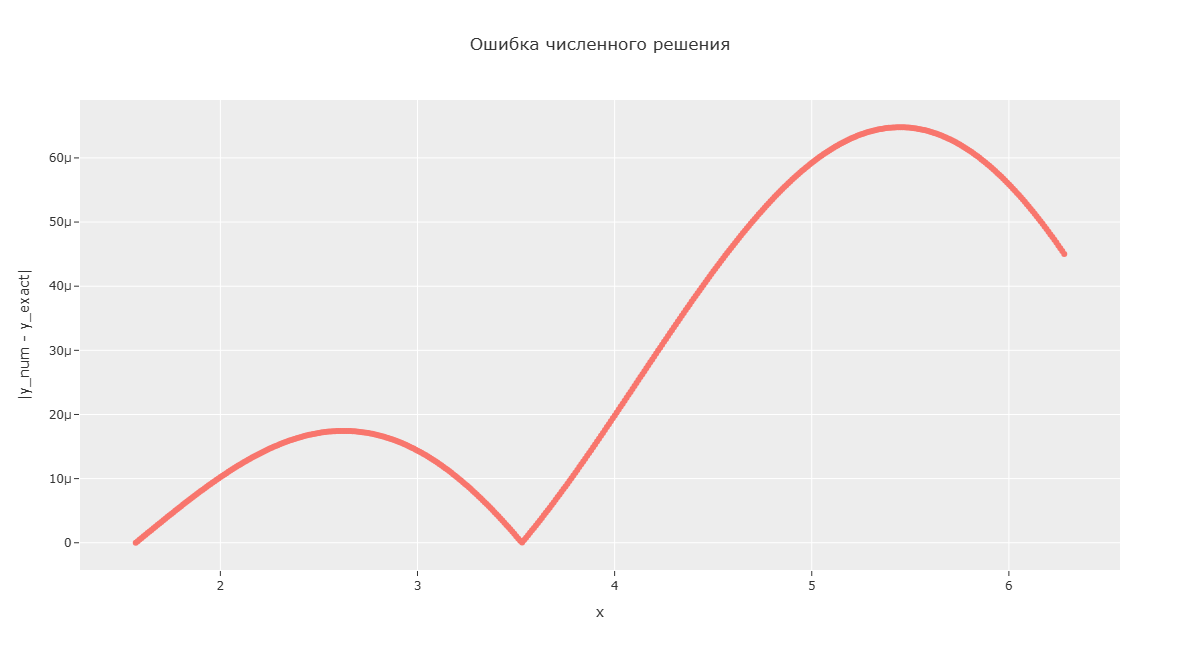
\includegraphics[width=0.9\linewidth]{../data/error.png}
				\caption{График ошибки}
				\label{fig:error}
			\end{framed}
		\end{figure}
		
		\begin{figure}[H]
			\centering
			\begin{framed}
				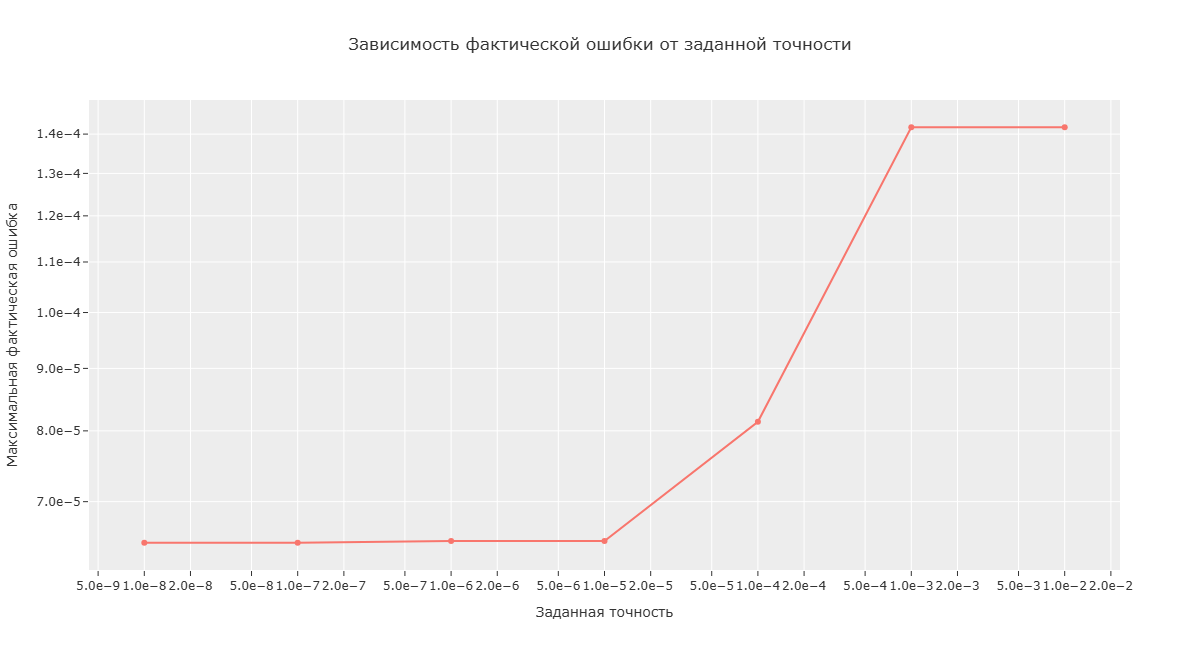
\includegraphics[width=0.9\linewidth]{../data/accuracy.png}
				\caption{График зависимости фактической ошибки от заданной точности}
				\label{fig:accuracy}
			\end{framed}
		\end{figure}
		
		
		\newpage
		\item Построен график решений: точного и метода \eqref{fig:solves}.
		
		Решение метода визуально совпадает с точным.
		
		\item Далее был построен график зависимости ошибки \eqref{fig:error} 
		
		Здесь уже можно пронаблюдать при каких значениях мы получаем соответствующую ошибку.
		
		\item И наконец был построен график зависимости ошибки от заданной точности \eqref{fig:accuracy}
		
		Чем меньше точность, тем меньше ошибка.
		
	\end{enumerate}
	
	
	
	%-------- the ninth point --------
	
	\newpage
	\section{\Large \underline{Выводы}}

	В ходе лабораторной работы был реализован
	метод Эйлера с пересчётом
	для решения задачи Коши
	для обыкновенного дифференциального уравнения
	первого порядка.

	В ходе вычислительных экспериментов установлено:
	
	\begin{itemize}
		\item численное решение хорошо совпадает
		с аналитическим;
		\item метод является устойчивым
		на рассматриваемом интервале;
		\item уменьшение заданной точности
		снижает ошибку;
	\end{itemize}
	
	Полученные результаты подтверждают
	корректность реализации метода
	и соответствуют теоретическим свойствам
	метода Эйлера с пересчётом.
	
	
	
\end{document}